\chapter{Introduction}
\label{ch:introduction}



\section{Introduction}

%\begin{itemize}
%
%    \item What is the subject of the study? Describe the
%        economic/econometric problem.
%
%    \item What is the purpose of the study (working hypothesis)?
%
%    \item What do we already know about the subject (literature
%        review)? Use citations: {\it \citet{Gallant:87} shows that...
%        Alternative Forms of the Wald test are considered
%        \citep{Breusch&Schmidt:88}.}
%
%    \item What is the innovation of the study?
%
%    \item Provide an overview of your results.
%
%
%    \item Outline of the paper:\\
%        {\it The paper is organized as follows. The next section describes %the
%        model under investigation. Section \ref{Sec:Literature Review} %reviews the up-to-date research works.
%        and Section \ref{Sec:Results} presents the results. Finally, %Section
%        \ref{Sec:Conc} concludes.}
%
%    \item The introduction should not be longer than 4 pages.
%
%\end{itemize}




\par The usage of Resource Description Framework \(RDF\) model is recently increasing in diverse fields in computer science, such as Big Data, Machine Learning, Data Science, Data Management, etc. The RDF data model helps computing machines in processing of "meta-data" which is data about data, especially those data about web resources. Moreover, such computing machines will be smarter to understand the data represented in different RDF serialization formats. 

Since the RDF model can facilitate  exchanging of data between software applications and it can be also serialized in multiple formats, such as Turtle\footnote{\href{https://www.w3.org/TR/turtle/}{Turtle}}, N-Triples\footnote{\href{https://www.w3.org/TR/n-triples/}{N-Triples}}, N3\footnote{\href{https://www.w3.org/TeamSubmission/n3/}{N3}}, JSON-LD	\footnote{\href{https://www.w3.org/2018/jsonld-cg-reports/json-ld/}{JSON-LD}}, RDF{/}XML\footnote{\href{https://www.w3.org/TR/rdf-syntax-grammar/}{RDF{/}XML}}, and RDF{/}JSON	\footnote{\href{https://dvcs.w3.org/hg/rdf/raw-file/default/rdf-json/index.html}{RDF{/}JSON}}, then its  quality and correctness needs to be proved before proceeding of any further processing. Most of available  parsers which check for syntax errors in RDF, fail to detect more than one error, especially those represented in Turtle or N-Triples serialization formats. Therefore, there is a need to have more powerful tools that help in listing all such errors or at least most of them.%todo needs to show most used formats  


This study was mainly  encouraged by the tremendous data representation and usage of either Turtle and N-Triples in different ontologies and in various sciences, as well as, to offer a solution to list most of syntax errors in RDF serialization formats, particularly Turtle and N-Triples. Hence, the intention of the study to afford a user-friendly syntax checker or parser. Such parser or syntax checker should give all errors can be detect inside such data.


\subsection{Motivation}

This study was motivated by several scenarios which require syntax checking of RDF data as an input and ensuring of its quality. To mention one of such scenarios, let's discuss an example shown in {\it Figure \ref{Fig:Motivation}}. The example describes a collaboration system for processing an input data, say for example to perform machine learning analysis. Of course,in a such case, a valid input data to the system is must. The input data is verified for further data processing. Most of the current existing systems  ensuring syntax-error-free RDF data, are stopped parsing at the first syntax error occurrence, as will be followed in Section \ref{Sec:Review}.
	\par
	To stop parsing when the first syntax error is found will introduce much complications. Assuming, the input RDF data contains, for example, 10 syntax errors. Normally, what is happing when an error is found, the system will proceed with no further processing, instead it will report error's existence in the inserted data. The reported error then should be corrected by the user, then after correction data will be send back for re-checking of data's syntax. To make it more complex, imagine that the user will do such correction process for 10 times (remember that data includes 10 errors). Then, what if the data contains hundreds or thousands of errors. 

	\begin{figure}[ht]
		\begin{center}
			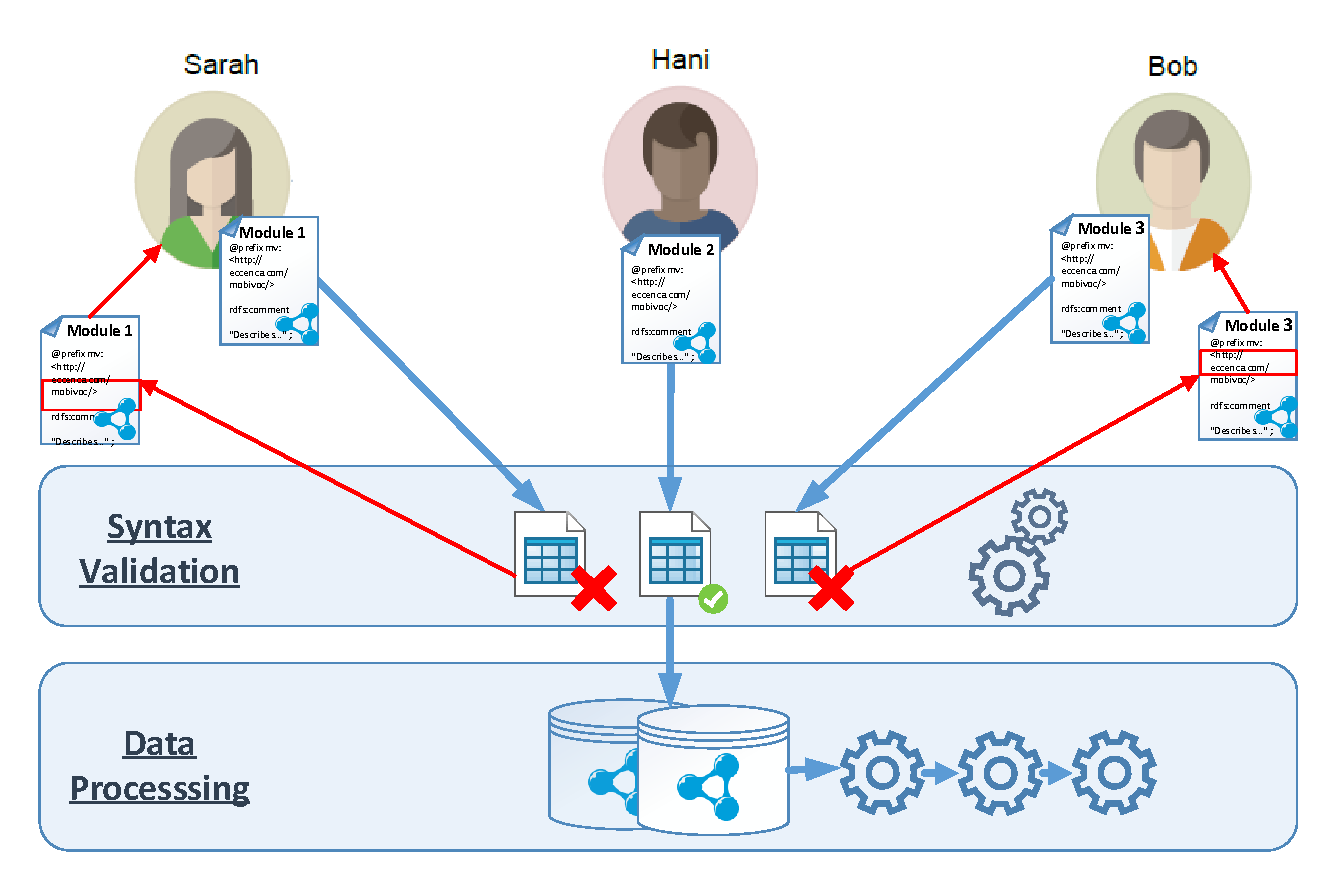
\includegraphics[scale=0.5,angle=0]{images/motivation}
			\caption{A motivation example of syntax checking of data before further processing}
			\label{Fig:Motivation}
		\end{center}
	\end{figure}

	let's dig deep to explain what is there in  {\it Figure \ref{Fig:Motivation}}, It is showing a flow of data from clients or users seeking further data processing. 3 persons are shown in this Figure, their names are Bob, Hani, and Sarah. All of them start with the first phase by sending the data to be syntacticly checked. The parser starts checking if there syntax errors of the input data, then if such data passed with no syntax errors, it can be forwarded for further phases, i.e. for data processing, otherwise, the input data will send back to the user to correct the errors. {\it Figure \ref{Fig:Motivation}} clearly shows that Sarah and Bob have syntax errors in their input data,then they got an error report, including found errors. In the meanwhile, Hani has received his data processed without getting such an error report, since his input data has no syntax errors. 
			\par
			This study has been encouraged by the illustrated example to find a suitable solution for such cases. The proposed solution will focus on producing a software program that can detect all or almost syntax errors that can be detected in the input data. 

%\section{Objectives}
\section{Proposed Problem } 	
The tackled problem in this study is to list all the detected syntax errors found in RDF files; in order to help ontology engineers and users to fix them in one shut. Such a list of errors provided in the output of the syntax checking phase will significantly assist to get rid of a loop of first error notification if multiple errors are found in the input data.  

\section{Challenges }
Before reaching the proposed solution, different methods have been tired to reach the objective. The main strategy was the continuation of parsing after error detection with reporting the detected error. The following 3 tools were individually tested: Jena RIOT API; RDF4J RIO API; and  N3 Parser %TODO need references.


\section {Contributions}
In this study, the research work set out to syntactically check RDF data. 
The main contributions of RDF-Doctor are:
\begin{enumerate}
	\item  {\bf Listing of detected syntax errors in RDF data:} it is a major goal and contribution where the intention to investigate RDF data, searching for syntax errors. RDF-Doctor is powered by ANTLR \cite{ANTLR:Website:Online}, a powerful parser generator, to establish an RDF parser that enable listing of all discovered syntax errors. By injecting of error production rules inside a grammar where our parser build based on. Once, the parser detects a combination of tokens from RDF input that match one of the error production rules, it sends an error notification for the error listener where error lists are stored.
	\item {\bf Reporting syntax errors with expressive messages:} it is of great benefits for debugging and user\_based error corrections when a parser provides friendly and helpful error messages to either normal users or ontology engineer. RDF-Doctor is not based on regular expression input recognition but its recognition is based on grammar rules, each rule represents either a group of correct syntax tokens or a group of incorrect ones. In case of the latter, RDF-Doctor has a predefined information for each error, then,  a customized error message, formulated in an expressive and convenient way is on-the-fly rendered.  
	\item {\bf Correcting some of detected syntax errors when applicable:} commonly syntax errors in well-know programming languages are those of missing a dot, adding more dots, or missing semicolon, similarly happens in RDF data. To limit annoying conflicts while error correction, A certain rule is set out to control the eligibility of an error to be corrected. The rule is the availability of a predefined error correction for such an error, otherwise, it cannot be corrected. For example, missing of a dot or semicolon are common while editing RDF data, then, RDF-Doctor can proficiently correct such errors, but in case of missing of a prefix declaration, decidedly, such an error is not corrected.     
\end{enumerate}

\section {Thesis Structure}
The thesis is organized as follows. The next chapter presents the preliminaries to shed light on the required background to understand what follows in the coming chapters. Chapter \ref{ch:related} reviews the up-to-date research works. Chapter \ref{ch:approach} describes the approach of the proposed solution. The implementation of the proposed solution is demonstrated in chapter \ref{ch:implementation} where its architecture and modules are exhibited.In chapter \ref{ch:evaluation}, the approach is evaluated  and the results are discussed . Finally, chapter
\ref{ch:conclusions} concludes this study.





